\subsection{Missing data}
\label{subsec:data-gaps}

\newcommand{\absentPerc}{75.9}
\newcommand{\absentEngPerc}{47.3}
\newcommand{\absentEngOneKPerc}{23.8}
\newcommand{\gapsPerc}{82.2}
\newcommand{\pregapsPerc}{78.0}
\newcommand{\midgapsPerc}{8.0}
\newcommand{\postgapsPerc}{14.1}

\newcommand{\midgapsPossPerc}{32.0}
\newcommand{\midgapsDomainsPerc}{55.0}
\newcommand{\lifespanNoGaps}{11.2}
\newcommand{\lifespanGaps}{16.8}

\newcommand{\numpresentdoms}{130,620}
\newcommand{\numabsentenglishdoms}{150,192}



\newcommand{\midgapNoRankPerc}{4}
\newcommand{\pregapNoRankPerc}{78}
\newcommand{\postgapNoRankPerc}{10}
\newcommand{\allgapNoRankPerc}{92}
\newcommand{\notgapNoRankPerc}{8}

\newcommand{\percSnapshotWithPrior}{85.3}

As with many large scale datasets, our dataset has missing data that should be considered, both in how it biases the data and how it affects analysis. There are four primary reasons a snapshot might be missing from our dataset.
\begin{enumerate}
    \item The website didn't exist at the time
    \item The website existed, but did not have a privacy policy
    \item The Wayback Machine did not crawl the homepage or the privacy policy
    \item Our crawler couldn't find or download the privacy policy
\end{enumerate}

The first and second reasons describe data that is non-existent, but is still worth considering -- our dataset will have more policies for websites that have existed for longer and had privacy policies. The third reason describes incomplete archiving. No archiving service can be complete, and our dataset inherits any biases from the Wayback Machine's archives. The final reason describes biases from our crawler; for example, our crawler may miss policies that do no use a standard link to direct users to their privacy policy.

It is critical to consider missing data -- we have no snapshots for \absentPerc\% of our candidate websites as described in section \ref{sec:sec:building-website-list}.

\subsubsection{Types of missing data}


\begin{figure}[t]
\centering
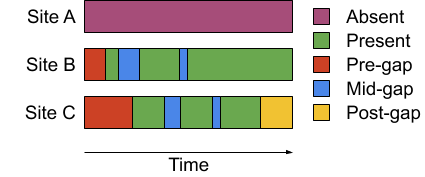
\includegraphics[width=1\columnwidth]{figures/gaps_diagram.png}
\caption{An illustration of the 4 types of missing data. Here we have 3 sites: Site A never appears in our dataset; Site B's first snapshot appears early and has some missing snapshots; Site C's first snapshot appears later, it has some missing snapshots, and has missing snapshots after it's last present snapshot}
\label{fig:missing_types}
\end{figure}

We categorize missing data into the following categories. For a missing snapshot, we categorize the missing data as follows (also illustrated in figure \ref{fig:missing_types}):
\begin{itemize}
    \item ``absent'': We have no privacy policies on any interval for that website.
    \item ``gap'': We do not have a privacy policy for that snapshot, but we do for a different interval for the same website
    \begin{itemize}
        \item ``pre-gaps'': We do not have a privacy policy for a prior interval, but we do for a later interval
        \item ``mid-gaps'': We have a privacy policy for a prior and a later interval.
        \item ``post-gaps'': We have a privacy policy for a prior interval, but not for a later interval
    \end{itemize}
\end{itemize}

\subsubsection{Absent Data}
We find that \absentEngPerc\% of English websites are absent. We are more likely to have a privacy policy for a popular website: \absentEngOneKPerc\% of the English websites that have been in the Alexa Top 1k are absent.

\subsubsection{Gaps}
%\gnote{86.1 of the snapshots do not have a gap between themselves and the previous snapshots from the same site. Let's not say midgaps are too common. And tell story from snapshots' point of view, not gaps. TODO: gunes rerun on non-dedup data}
Once we remove all absent websites, the missing data that are left are gaps.

We find that, for non-absent websites, \gapsPerc\% of possible snapshots are a gap. Of these gaps, \pregapsPerc\% are pre-gaps, \midgapsPerc\% are mid-gaps, and \postgapsPerc\% are post-gaps. The large scale of pre-gaps is expected -- after all, most websites have not existed since 1997, and many websites are not archived by Internet Archive, especially before they gain popularity.

Even with perfect archiving, we expect pre-gaps and post-gaps would still be expected, as websites come and go. Therefore, we believe mid-gaps to be the most important gaps to consider. We found that \percSnapshotWithPrior\% of snapshots that are not the first snapshot for a site are have another snapshot immediately before them. We found that \midgapsDomainsPerc\% of websites have at least one mid-gap. Longer-lived websites are also more likely to have gaps -- websites for which we have no gaps live an average \lifespanNoGaps~intervals, compared to \lifespanGaps~intervals for websites with gaps.

A mid-gap likely reflects a failure in collection rather than a lack of existence, and most sites have a midgap. We therefore recommend that users of the dataset consider imputing mid-gaps with a policy from a preceding or succeeding interval on the same website. The choice of which interval to draw from, and if imputation is needed, depends on the particular research question.

Overall stats (e.g. perc of possible policies that are gaps)
Only do overall stats for websites that have a rank
Gap distribution based on w-i pairs with rank
% of websites that have pre/mid/post gaps?
Focus on midgaps, only briefly touch on pre/post gaps
median number of mid-gaps
Optional: how long do mid-gaps run?
Longevity: median(last\_year - start\_year)


{\textbf{Website popularity.}}
In order to identify if Alexa rank has any bias effects on gaps, we show how the percentage of snapshots that are gaps changes with rank in figure \ref{fig:rank_absent}. We can see that pre-gaps and post-gaps are more common among high-ranked snapshots, whereas mid-gaps frequency does not seem to vary much with rank. Among snapshots without a rank, just \midgapNoRankPerc\% of snapshots are midgaps, \pregapNoRankPerc\% are pre-gaps, \postgapNoRankPerc\%  are post-gaps, leaving just \notgapNoRankPerc\% of snapshots present. This suggests that pre- and post-gaps are connected with a decline in rank, unlike mid-gaps, supporting the hypothesis that pre- and post-gaps are partially caused by low website popularity or non-existence.

\begin{figure}[t]
\centering
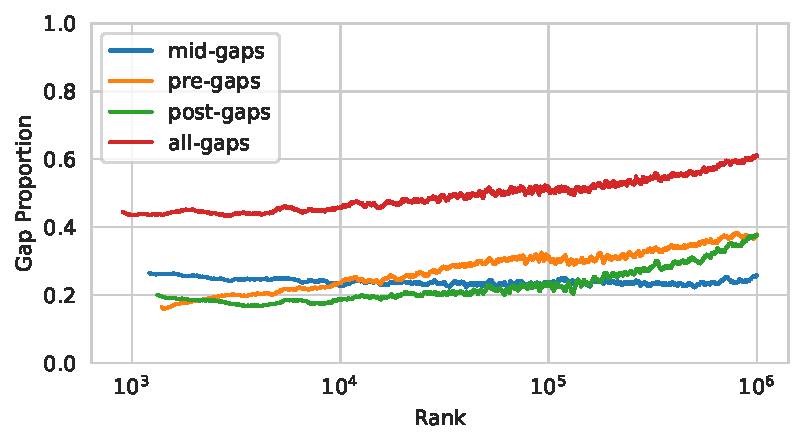
\includegraphics[width=1\columnwidth]{figures/gap_rank_absent.pdf}
\caption{The proportion of snapshots that are gaps as a function of rank. Proportion is calculated as the smooth moving average over the 10,000 neighboring snapshots. Snapshots without a rank are omitted. \rnote{Consider removal}}
\label{fig:rank_absent}
\end{figure}

% \begin{figure}[t]
% \begin{subfigure}[t]{0.45\textwidth}
% \centering
% 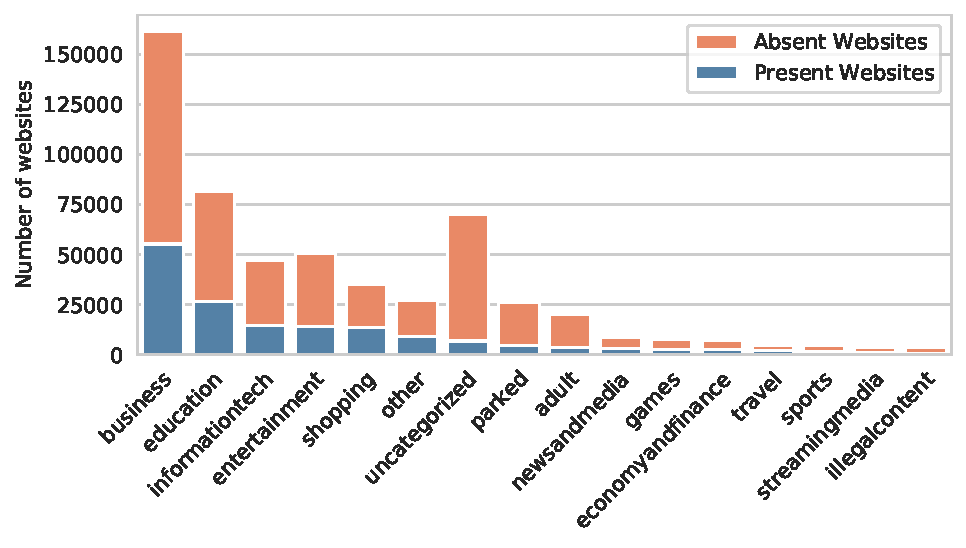
\includegraphics[width=1\columnwidth]{figures/category_dist.pdf}
% \caption{The distribution of website categories within our dataset.}
% \label{fig:cat_dist}
% \end{subfigure}
% \hfill
% \begin{subfigure}[t]{0.45\textwidth}
% \centering
% 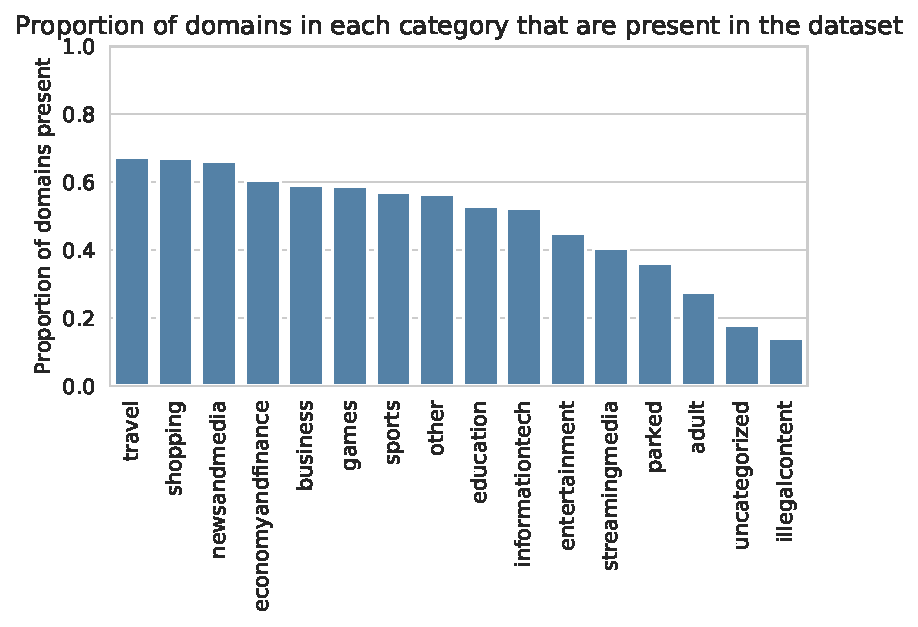
\includegraphics[width=1\columnwidth]{figures/category_missing_perc.pdf}
% \caption{The proportion of English-language websites for which we have privacy policies, grouped by category.}
% \label{fig:cat_prop}
% \end{subfigure}

% \caption{The representation of categories in our dataset. ``Other'' is composed of the 27 least frequent categories for English language websites. Policies which belong to multiple categories are counted once per category. Policies with no listed categories are added to the ``uncategorized'' category.\gnote{Think we should go back to the combined category plot or omit 6-b to save space. We can mention the uneven success across categories in the text}}
% \label{fig:categories}
% \end{figure*}

\begin{figure}[t]
\label{fig:cat_dist}
\centering
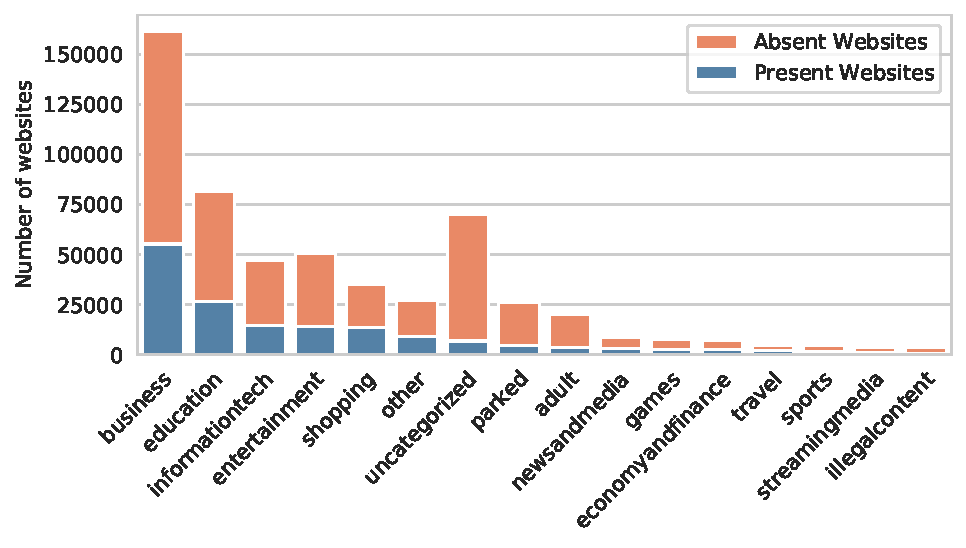
\includegraphics[width=1\columnwidth]{figures/category_dist.pdf}

\caption{The distribution of website categories for present and missing sites. ``Other'' is composed of the 27 least frequent categories for English language websites. Policies which belong to multiple categories are counted once per category. Policies with no listed categories are added to the ``uncategorized'' category.\rnote{We removed the double plot to save space. Should we label orange ``total'' or as-is?}}
\label{fig:categories}
\end{figure}


{\textbf{Distribution of website categories.}}
We further examine the website categories for which we have the best coverage. We collected category data from Webshrinker~\cite{Webshrinker}, which provides a domain category lookup API.
We also collected a small sample of category data from Alexa Web Information Services, but we found the data to be sparse compared to Webshrinker~\cite{awis}; these findings are consistent with those of other researchers~\cite{mathur2019dark}.
Because category data is not available historically from Webshrinker, we made the assumption that categories are constant across time. We collected category data for the \numpresentdoms~websites in our dataset and the \numabsentenglishdoms~websites with English homepages that were at one point in the Alexa Top 100k.
In Figure~\ref{fig:cat_dist} we show the distribution of categories within our dataset and categories that are absent. We see that just a few categories dominate most of the dataset. We also see that for most categories, we capture 40\% or more of the top 100k, English language websites.
However, some categories are strongly underrepresented in our dataset, such as illegal content\footnote{Illegal content is primarily copyright-infringing content}.

\subsection{Evaluating data quality}
\label{subsec:ppot:failure-analysis}

To ensure our dataset was of high quality, we manually investigated causes of failure (i.e., homepages where the crawler did not extract privacy policy text). We started with 5,223,228 homepage snapshots, and our crawler was able to download 1,292,420 privacy policy snapshots (24\%).
Downloads of privacy policies corresponding to the other 3,930,808 homepage snapshots failed due to various causes which we list in Table~\ref{tab:failure-cause}. While the high frequency of absent policies may be counter-intuitive, we found that only about 2\% of missing policies were attributable to crawler limitations.

The most common cause for a missing privacy policy, by far, was the crawler loading an archived homepage but failing to identify a privacy policy link.
The next most common cause was a~\emph{blank homepage}, where the crawler could not extract any text. Another recurring issue was that, though we had attempted to filter our non-English sites before the crawl, some homepage snapshots were classified as non-English.

To investigate the root causes of crawler failures, we manually analyzed 100 random snapshots for each of the most common crawl failures.
The main takeaways are:
only 4 of 100 homepages where the crawler did not identify a privacy policy link actually had a privacy policy link. Only 3 of 100 homepages detected as \emph{blank} contained a privacy policy link, while 13 contained some text in a separate frame--- typically old webpages. We further explore the relation between the snapshot age and crawl success in 
Section~\ref{subsec:ppot:data-overview}.

In sum, the overwhelming majority of crawl failures were attributable to homepage snapshots that did not contain a policy link, were not archived by the Wayback Machine (e.g., due to \texttt{robots.txt} rules), or were in a language other than English. The missing privacy policies that are attributable to limitations of the crawler are about 2\% of all snapshots (4\% of 44.7\% + 3\% of 7.3\%).


\begin{table}[t]
\centering
\resizebox{0.9\columnwidth}{!}{%
\begin{tabular}{@{}lrr@{}}
\toprule
\textbf{Failure cause}                           & \textbf{Count} & \textbf{Percent} \\ \midrule
No privacy policy link found on homepage         & 2,336,849      & 44.7\%       \\
Homepage detected as blank                        & 383,337       & 7.3\%      \\
Non-English homepage                             & 310,563        & 5.9\% \\
Policy page is not archived in this interval     & 271,736        & 5.2\%\\
Out-of-interval redirection for homepage         & 158,727        & 3.0\%\\
\bottomrule
\end{tabular}%
}
\caption{The five most common causes for the crawler to not download a privacy policy for a homepage. Out-of-interval redirection (row 5) means our crawler was redirected by the Wayback Machine to a snapshot in a different interval.}
\label{tab:failure-cause}
\end{table}

